\documentclass[12pt]{article}
\usepackage{geometry}
\usepackage{amsmath} 
\usepackage{amsthm}
\usepackage{amsfonts}
\usepackage{cases}
\usepackage{graphicx}
\usepackage{caption}
\usepackage{subcaption}
\usepackage{gauss}
\usepackage{tikz}
\usetikzlibrary{positioning}
\usetikzlibrary{matrix}
\usepackage{tkz-graph}
\usetikzlibrary{arrows}
% set arrows as stealth fighter jets
\tikzset{>=stealth}


\def\dotp#1#2{\langle#1,#2\rangle}
\def\ss#1#2{\sum_{#1=1}^{#2}}
\def\lam{\lambda}
\def\vec#1{\{#1_1,#1_2\ldots#1_n\}}
\def\es#1#2{{\bf Exercise #1}\\~{\it Solutions:}\\~#2\\[1em]}
\def\ep#1#2{{\bf Exercise #1}\\~{\it Proof:}\\~#2\\[1em]}
\def\inn#1#2{(#1): #2\\[0.5em]}
\def\ff#1#2{\frac{#1}{#2}}
\def\cgu#1{\overline{#1}}
\def\ran#1{{\rm ran}\,#1}
\def\ker#1{{\rm ker}\,#1}
\def\tr#1{{\rm tr}\left(#1\right)}
\def\dotr#1#2{\dotp{#1}{#2}_{\rm tr}}
\def\lr#1#2#3{\left#1#3\right#2}
\newcommand{\R}{\mathbb{R}}
\newcommand{\bb}[1]{\mathbb{#1}}
\newcommand{\eq}[1]{\begin{align*}#1\end{align*}}
\newcommand{\mm}[1]{\begin{pmatrix}#1\end{pmatrix}}

\def\sg{\sigma}
\def\ct{\cos{\theta}}
\def\st{\sin{\theta}}
\def\sq#1{\sqrt#1}
\newcommand{\B}{\mathcal{B}}

\linespread{1.4}
\geometry{a4paper,centering,scale=0.8}
\rmfamily 
\normalsize
\setlength{\parindent}{0em}

\begin{document} 
\begin{flushleft}
  Junlong Gao 5133709126\\ 
  Prof.  Hohberger\\ 
  VV285 Assignment 3\\
  \today 
\end{flushleft}

\es{1}{
	\inn{i}{
		\begin{align*}
		\dotp{x}{Ay}&=\ss{i}{n}x_i\ss{j}{n}y_ja_{ij}=\ss{j}{n}x_j\ss{i}{n}y_ia_{ji}=\ss{i}{n}y_i\ss{j}{n}x_ja_{ji}=\dotp{A^Tx}{y}
		\end{align*}
	}
	\inn{ii}{
		\[
		\left({(AB)}^T\right)_{ij}=\left(AB\right)_{ji}=\ss{k}{n}a_{jk}b_{ki}=\ss{k}{n}b_{ki}a_{jk}
		\]
		Since we only need to exchange the role of row index and column index.\\
		Also, consider that
		\[
		\left({B}^T\!{A}^T\right)_{ij}=\ss{k}{n}b_{ki}a_{jk}
		\]
		Again, we exchanged the role of row and column index.\\
		Since by above each entry is equal
		\[
		{(AB)}^T={B}^T\!{A}^T
		\]
		}
	\inn{iii}{
		Consider 
		\[
			A=\begin{pmatrix}
			1&2\\
			2&1
			\end{pmatrix}
			\quad
			A^T=\begin{pmatrix}
			1&2\\
			2&1
			\end{pmatrix}
		\]Thus $A=A^T$.
	}
	\inn{iv}{
		Given $A$ is orthogonal, then
		\[
		I=A^{-1}A=A^TA
		\]
		}
		Since the $i$th row of $A^T$ is the $i$th column of $A$, denoted by $A_i$ the above identity shows
		\[
		A_iA_j=I_{ij}=\delta_{ij}
		\]
		Therefore the column vectors of an orthogonal matrix  are othonormal.
}
\es{2}{
	\inn{a}{
		Consider
		\[
		A=\begin{pmatrix}
		\ff{\sqrt3}{2}&\ff{1}{2}\\
		\ff{1}{2}&-\ff{\sqrt3}{2}
		\end{pmatrix}
		\]
		We can read off that $A=A^T$ and by calculation we have 
		\[
		A^{-1}=\begin{pmatrix}
		\ff{\sqrt3}{2}&\ff{1}{2}\\
		\ff{1}{2}&-\ff{\sqrt3}{2}
		\end{pmatrix}=A
		\]
	}
	\inn{b}{
		Consider
		\[
		B=\begin{pmatrix}
		\ff{\sqrt6}{3}&-\ff{\sqrt3}{3}\\
		\ff{\sqrt3}{3}&\ff{\sqrt6}{3}
		\end{pmatrix}
		\]
		And 
		\[
		B^T=\begin{pmatrix}
		\ff{\sqrt6}{3}&\ff{\sqrt3}{3}\\
		-\ff{\sqrt3}{3}&\ff{\sqrt6}{3}
		\end{pmatrix}
		\]
		}
		Then one can verify that $BB^T=I$, i.e. $B^{-1}=B^T$.
}
\es{3}{
	\inn{i}{
		Notice that $Ae_j=A_j$ if we apply the equivalence of matrix and linear map by theorem 1.5.3, $A_j$ being the $j$th column of the matrix. Now since $A_j=\ss{i}{n}a_{ij}e_i$, by the linearity of  inner product, we see that
		\[
		\dotp{e_i}{Ae_j}=\ss{i}{n}a_{ij}\dotp{e_i}{e_j}=\ss{i}{n}a_{ij}\delta_{ij}=a_{ij}=A_{ij}
		\]
	}
	\inn{ii}{
	\[
	\partial_{ij}=\dotp{e_i}{\partial e_j}=\int_{-1}^{1}(j-1)x^{i-1+j-2}\,dx=\ff{j}{i+j-2}\left(1-{(-1)}^{i+j-2}\right)
	\]
	for $j>1$, and $\partial_{1,1}=0$
	}
	\inn{iii}{
	Consider the following diagram:
	\[
	\begin{tikzpicture}
		\SetGraphUnit{3} 
		\GraphInit[vstyle=Empty] 
		\tikzset{VertexStyle/.append style = {shape=rectangle,inner sep=0pt}} 
		\Vertex[L= $\mathbb{F}^n$ ]{1} 
		\EA[unit=3.2,L= $\mathbb{F}^n$ ](1){2} 
		\NO[unit=2.5,L=$V$](1){4} 
		\NO[unit=2.5,L=$V$](2){3}
		\begin{scope}[every node/.style={midway},>=latex']  
		  \draw[->] 	(4)--(3) node [above] {$L$};
		  \draw[->]        (3)--(2) node [right] {$\varphi_A$} ;
		  \draw[->]        (1)--(2) node [below] {$\varphi_A\!\circ\!L\!\circ\!{\varphi_A}^{-1}$};
		  \draw[->]        (4)--(1) node [left]  {$\varphi_A$};
		\end{scope}
	\end{tikzpicture} 
	\]
	where $\varphi_A$ is the coordinate isomorphism: $V\cong\mathbb{F}^n$.\\
	Now we consider the induced map 
	\[
	\varphi_A^{*}:\quad L\mapsto\varphi_A\circ L\circ{\varphi_A}^{-1} 
	\]
	whose image is linear since
	\eq{
	\varphi_A\circ (aL+bT)\circ{\varphi_A}^{-1}(v)&=\varphi_A( (aL+bT)({\varphi_A}^{-1}(v)))\\
	&\quad=\varphi_A( aL({\varphi_A}^{-1}(v))+bT({\varphi_A}^{-1}(v)))\\
	&\quad=a\varphi_A(L({\varphi_A}^{-1}(v)))+b\varphi_A(T({\varphi_A}^{-1}(v))))\\
	&\quad\quad=a\varphi_A\circ (L)\circ{\varphi_A}^{-1}(v)+b\varphi_A\circ (T)\circ{\varphi_A}^{-1}(v)
	}
	Also it's bijective since it's injective, for a none zero mapping $L$, we have $L(v)$ none zero for some  $v$, and $\varphi_A$ and $\varphi_A$ is injective thus ${\varphi_A}\circ L\circ \varphi_A^{-1}(v)={\varphi_A}^{-1}(L\circ (\varphi_A(v)))\neq0$. And it's surjective for given an image $L$ the pre-image can be found: ${\varphi_A}^{-1}\circ L\circ \varphi_A$.\\
	Therefore the coordinate isomorphism induces a isomorphism: $\mathcal{L}(V,V)\cong \mathcal{L}(\mathbb{F}^n,\mathbb{F}^n)$. Since $\mathcal{L}(\mathbb{F}^n,\mathbb{F}^n)\cong{\rm Mat}(n\times n,\mathbb{F})$ we know $\mathcal{L}(V,V)\cong{\rm Mat}(n\times n,\mathbb{F})$ as desired.
	}
}
\ep{4}{
	\inn{i}{
	Uniqueness:
	Since a finite-dimensional inner product space is isomorphic to a $\mathbb{R}^n$, pick a orthonormal basis system (in column vector) and note that for a given $A\in\mathcal{L}(V,V)$
	\[
	\dotp{e_i}{Ae_j}=\ss{k}{n}\dotp{e_i}{a_{kj}e_k}=a_{ij}
	\]
	And
	\[
	\dotp{A^*e_i}{e_j}=\ss{k}{n}\dotp{a^*_{ki}e_k}{e_j}=\overline{a^*_{ji}}
	\]
	Since they are equal, this determines $A^*$ uniquely:
	\[
	\overline{a^*_{ji}}=a_{ij}
	\]
	Existence: take the $A^*$ we formed above, we know that for any $x,y\in V$, by basis expansion:
	\[
	\dotp{x}{Ay}=\ss{i}{n}\ss{j}{n}x_iy_j\dotp{e_i}{Ae_j}=\ss{i}{n}\ss{j}{n}x_iy_j\dotp{A^*e_i}{e_j}=\dotp{A^*x}{y}
	\]
	Since inner product is invariant under component addition.\\
	}
	\inn{ii}{
	By (i) we know that $\overline{a^*_{ji}}=a^*_{ji}=a_{ij}$ since it's a real number, then $A^*=A^T$. And for $V=\mathbb{C}^n$, by (i) it's clear that $\overline{(a^*_{ij})}=a_{ji}$ taken conjugation and transpose (row and column exchange): $A^*=\overline{A^T}$
	}
	\inn{iii}{
	Consider
	\[
	\begin{pmatrix}
	1&1+i\\
	1-i&1
	\end{pmatrix}
	\]
	}
	\inn{iv}{
	Note that for $L\in\mathcal{L}(V,V)$
	\begin{align*}
	&{\rm ran}\,L=\{v\in V:\exists\,{u\in V}\quad v=Lu\}\\
	&{\rm ker}\,L=\{v\in V:Lv=0\}\\
	&M^{\perp}=\{v\in V:\forall\,m\in M\quad\dotp{m}{v}=0\}
	\end{align*}
	Now, given that $w\in{(\ran{A})}^{\perp}$ i.e. $\forall\,v\in V$ $\dotp{w}{Av}=0$
	\eq{
	&\iff \forall\, v\in V,\quad\dotp{A^*w}{v}=\dotp{w}{Av}=0\\
	&\iff A^*w=0\quad\hbox{since we can choose $v$ to be each orthonormal  basis}\\
	&\iff w\in\ker{A^*}
	}
	The equivalence in the deduction shows that ${(\ran{A})}^{\perp}=\ker{A^*}$.\\
	Next, we first settle a lemma:\\
	Given finite dimensional subspace $W$ of finite dimensional vector space $V$, if $\{b_1,b_2,\ldots,b_r\}$ is a  orthonormal basis of $W$ and by extension theorem $\{b_1,b_2,\ldots,b_r,\ldots,b_n\}$ is a orthonormal basis of $V$ (using Gram-Schmidt Orthonormalization process), then $W^{\perp}$ has a basis of $\{b_{r+1},b_{r+2},\ldots,b_n\}$.\\
	\hbox{\it Proof}:\\
	For $\forall u\in$ span $\{b_{r+1},b_{r+2},\ldots,b_n\}$, by reading off the coefficients of $u$ we see that $\dotp{u}{v}=0$, $\forall v\in W$, i.e., $u\in W^{\perp}$. On the other hand, we see that if $u\in W^{\perp}$ then $\dotp{u}{b_i}=0$ for $i=1,2\ldots r$, therefore $u$ is a linearly combination of $b_{r+1},b_{r+2},\ldots,b_n$, i.e., $u\in$ span $\{b_{r+1},b_{r+2},\ldots,b_n\}$, then we are done.\\
	By doubly using the above lemma we see that $M=M^{\perp\perp}$. Also from definition we see that $A^{**}=A$. Then ${(\ran{A^*})}^{\perp}=\ker{A^{**}}$ from previous result implies $(\ran A^*)^{\perp\perp}={\ker{A}}^{\perp}$ which is ${\ker{A}}^{\perp}=\ran A^*$.
	}
}
\ep{5}{
	\inn{i}{
	Existence: Since $V=M\oplus N$, define mapping $P$:
	\[
	\forall v\in V:\, P(v)=u,\qquad \hbox{where } v=u+w, u\in M, w\in N
	\]
	since the sum is direct, the above decomposition is unique and $P$ is well defined.\\
	Now it remains to be shown that $\ran P=M$ and $\ker P=N$. From definition we immediately see
	 that $\ran P\subset M$, also $\forall u\in M$, $u=Pu\in \ran P$ , thereby $ M\subset\ran P$, we conclude that
	 $\ran P=M$.\\
	 Again from definition we see that $N\subset \ker P$, also if $v\in \ker P$, then $Pv=0$, we know that $v$ has decomposition $v=0+w$, $v=w\in N$, and this shows that $\ker P\subset N$, we conclude that $\ker P=N$.\\
	 Uniqueness: Suppose for another mapping satisfying the condition: $\forall v\in V, P'v=P'u+P'w=u'+0$, where $v=u+w$ is the unique decomposition $u\in M$, $w\in N$, we have: $P'^2u=P'u=P'u'$ since $P'^2=P'$, we have $P'(u-u')=0$, which implies $u-u'\in\ker P'=N$, yet note that from our assumption $u,u'\in M$, which means $u-u'\in M$. Now, since the sum is direct, $M\cap N=\{0\}$ we conclude that $u=u'$. Thus $P'=P$ coincide everywhere and the mappings are identical.
	}
	\inn{ii}{
	For $\forall v\in V$ can be written uniquely as
	\[
	v=u+v-u,\quad \hbox{where $u=Pv$}
	\]
	and it's clear $u\in \ran P$. It remains to be shown that $u-v\in \ker P$:
	\[
	P(v-u)=Pv-Pu=P^2v-Pu=P(Pv-u)=P(u-u)=0
	\]
	Thus by lemma $1.2.27$ we know that $V=\ran P\oplus \ker P$ 
	}
	\inn{iii}{
	Consider $a,b\in\R$ and $x,y\in\R^n$
	\eq{
	P(ax+by)=\ss{i}{m}\dotp{e_i}{ax+by}e_i=a\ss{i}{m}\dotp{e_i}{x}e_i+b\ss{i}{m}\dotp{e_i}{y}e_i=aPx+bPy
	}
	And
	\[
	P^2x=P\left(\ss{i}{m}\dotp{e_i}{x}e_i\right)=\ss{i}{m}\dotp{e_i}{x}\ss{j}{m}\dotp{e_i}{e_j}e_j=\ss{i}{m}\dotp{e_i}{x}e_i=Px
	\]
	Thus $P^2=P$.\\
	Also, we notice that $\ran P\subset M$ from definition in question and $M\subset\ran P$ since $w\in M$ we have $w=Pw\in \ran P$ thereby $M=\ran P$  and we proceed as ${\ran P}^{\perp}=M^{\perp}$:
	\eq{
	    &\forall w\in\,{M}^{\perp}\\
	\iff&\,\forall\,x\in\,{M}\quad\dotp{w}{x}=0\\
	\iff&\,\forall\,x\in\,{M}\quad\ss{i}{r} \dotp{w}{e_i}x_i=0\\
	\iff&\,\,\dotp{w}{e_i}=0\quad{\rm for}\,i=1,2,\ldots r\quad\hbox{(if we pick $x_i=1$ and others to be $0$)}\\
	\iff&\,Pw=\ss{i}{m}\dotp{e_i}{w}e_i=0\quad\hbox{(since all $e_i$ are independent)}\\
	\iff&\,w\in\ker{P}
	}
	The equivalence in the deduction shows that ${\ran P}^{\perp}=\ker{P}$.
	}
	\inn{iv}{
	\[
	\dotp{x}{Py}=\dotp{x}{\ss{i}{m}\dotp{e_i}{y}e_i}=\ss{i}{n}\dotp{x}{e_i}\dotp{e_i}{y}=\ss{i}{n}\dotp{e_i}{x}\dotp{e_i}{y}=\dotp{\ss{i}{m}\dotp{e_i}{x}e_i}{y}=\dotp{Px}{y}
	\]
	And
	\[
	\dotp{x}{Py}=\dotp{P^*x}{y}\quad\hbox{$x,y\in V$}
	\]
	from previous exercise. In particular, choose $x,y$ to be $e_i,e_j$, then the $P_{ji}=P^*_{ji}$ for all $i,j=1,2\cdots,n$. Thus $P=P^*$.
	Other the other hand, from Exercise 4 iv), we see that $(\ker P)^{\perp}=\ran P^*$ and itself is a projection, thereby from previous result it's a orthogonal projection.
	}
	\inn{v}{
	\[
	P_1=\mm{1&0\\0&0},P_2=\mm{1/2&1/2\\1/2&1/2},P_3=\mm{1&-1\\0&0}.
	\]
	}
}
\ep{6}{
	\inn{i}{
	Since we are only interested in the diagonal elements, we see that
	\[
	\ss{i}{n}{(AB)}_{ii}=\ss{i}{n}\ss{j}{n}a_{ij}b_{ji}=\ss{j}{n}\ss{i}{n}a_{ji}b_{ij}=\ss{i}{n}\ss{j}{n}b_{ij}a_{ji}=\ss{i}{n}{(BA)}_{ii}
	\]
	Thus $\tr{AB}=\tr{BA}$\\
	Let 
	\eq{
	A=
	\begin{pmatrix}
				1 & 1 \\
				0 & 1
	\end{pmatrix}
	\quad
	B=
	\begin{pmatrix}
				1 & 0 \\
				1 & 1
	\end{pmatrix}
	\quad
	AB=
	\begin{pmatrix}
				2 & 1 \\
				1 & 1
	\end{pmatrix}
	}
	we may read off that $\tr{A}=\tr{B}=1$ yet $\tr{AB}=2\ne\tr{A}\tr{B}$
	}
	\inn{ii}{
	(conjugate symmetric:) 
	\eq{
	\dotr{B}{A}&=\tr{\cgu{B^T}A}=\tr{\cgu{B}^TA}=\tr{\lr(){\cgu{B}A^T}^T}=\tr{\cgu{B}A^T}\\
	&\quad=\tr{\cgu{\lr(){\cgu{A^T}B}}}=\cgu{\tr{\cgu{A^T}B}}=\cgu{\dotr{A}{B}}
	}
	(linearity in second component:) 
	\eq{
	\dotr{A}{xB+yC}=&\tr{A^*\lr(){xB+yC}}=\tr{xA^*B+yA^*C}\\
	&\quad =x\tr{A^*B}+y\tr{A^*C}=x\dotr{A}{B}+y\dotr{A}{C}
	}
	For any $x,y\in\R$.\\
	(Positive definite)
	\[
	\dotr{A}{A}=\tr{\cgu{A^T}A}=\ss{i}{n}\ss{j}{n}{|a_{ji}|}^2\ge0
	\]
	which can be $0$ if and only if $A=0$, as desired.\\
	Thus the induced norm takes on the form
	\[
	\|A\|_{\rm tr}=\sqrt{\ss{i}{n}\ss{j}{n}{|a_{ji}|}^2}
	\]
	}
	\inn{iii}{
	They are linearly independent, for if we have
	\[
	x\sg_0+y\sg_1+z\sg_2+w\sg_3=0
	\]
	we are left with
	\eq{
	&x+w=0\\
	&y-zi=0\\
	&y+zi=0\\
	&x-w=0
	}
	having only trivial solution, thus the spin matrixes are linearly independent.\\
	Now, we notice that, if considering six different product
	\eq{
	&\dotr{\sg_0}{\sg_1}=\tr{\sg_0^*\sg_1}=	
	\tr{
	\begin{pmatrix}
	1&0\\
	0&1
	\end{pmatrix}
	\begin{pmatrix}
	0&1\\
	1&0
	\end{pmatrix}
	}
	=\tr{\begin{pmatrix}
	0&1\\
	1&0
	\end{pmatrix}}
	=0\\
	&\dotr{\sg_0}{\sg_2}=
	\tr{
	\begin{pmatrix}
	1&0\\
	0&1
	\end{pmatrix}
	\begin{pmatrix}
	0&-i\\
	i&0
	\end{pmatrix}
	}
	=0\\
	&\dotr{\sg_0}{\sg_3}=
	\tr{
	\begin{pmatrix}
	1&0\\
	0&1
	\end{pmatrix}
	\begin{pmatrix}
	1&0\\
	0&-1
	\end{pmatrix}
	}
	=0\\
	&\dotr{\sg_1}{\sg_2}=
	\tr{
	\begin{pmatrix}
	0&1\\
	1&0
	\end{pmatrix}
	\begin{pmatrix}
	0&-i\\
	i&0
	\end{pmatrix}
	}
	=0\\
	&\dotr{\sg_1}{\sg_3}=
	\tr{
	\begin{pmatrix}
	0&-i\\
	i&0
	\end{pmatrix}
	\begin{pmatrix}
	1&0\\
	0&-1
	\end{pmatrix}
	}
	=0\\
	&\dotr{\sg_2}{\sg_3}=
	\tr{
	\begin{pmatrix}
	0&-i\\
	i&0
	\end{pmatrix}
	\begin{pmatrix}
	1&0\\
	0&-1
	\end{pmatrix}
	}
	=0
	}
	Also, we see that 
	\eq{
	&\dotr{\sg_0}{\sg_0}=\tr{\sg_0^*\sg_0}=	
	\tr{
	\begin{pmatrix}
	1&0\\
	0&1
	\end{pmatrix}
	\begin{pmatrix}
	1&0\\
	0&1
	\end{pmatrix}
	}
	=1\\
	&\dotr{\sg_1}{\sg_1}=	
	\tr{
	\begin{pmatrix}
	0&1\\
	1&0
	\end{pmatrix}
	\begin{pmatrix}
	0&1\\
	1&0
	\end{pmatrix}
	}
	=1\\
	&\dotr{\sg_2}{\sg_2}=	
	\tr{
	\begin{pmatrix}
	0&-i\\
	i&0
	\end{pmatrix}
	\begin{pmatrix}
	0&-i\\
	i&0
	\end{pmatrix}
	}
	=1\\
	&\dotr{\sg_3}{\sg_3}=	
	\tr{
	\begin{pmatrix}
	1&0\\
	0&-1
	\end{pmatrix}
	\begin{pmatrix}
	1&0\\
	0&-1
	\end{pmatrix}
	}
	=1
	}
	thereby making it an orthonormal basis.
	}
}
\ep{7}{
	In polar coordinate system:
	\[
	x=
	\begin{pmatrix}
				\rho \cos\theta \\
				\rho \sin\theta
	\end{pmatrix}
	\]
	Then 
	\eq{
	x'=\mathcal{R}(\varphi)(x)=
	\begin{pmatrix}
				\rho \cos\theta \cos\varphi-\rho \sin\theta \sin\varphi \\
				\rho \cos\theta \sin\varphi-\rho \sin\theta \cos\varphi
	\end{pmatrix}
	=
	\begin{pmatrix}
				\rho \cos(\theta+\varphi) \\
				\rho \sin(\theta+\varphi)
	\end{pmatrix}
	}
	Now, geometrically, this transformation takes $\theta$ into $\varphi+\theta$ in a counter-clockwise direction, with length preserved. Thereby the transformation $\mathcal{R}(\varphi)$ rotates $x$ by the angle of $\varphi$ in a counter-clockwise direction.
}
\es{8}{
	Consider the commutative diagram:
	\[
	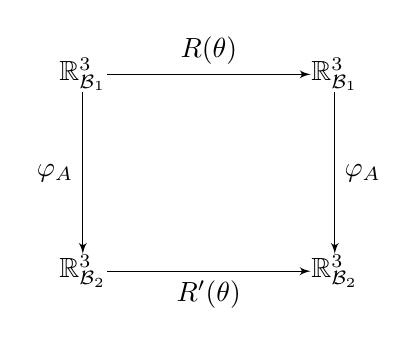
\begin{tikzpicture}
		\SetGraphUnit{3} 
		\GraphInit[vstyle=Empty] 
		\tikzset{VertexStyle/.append style = {shape=rectangle,inner sep=0pt}} 
		\Vertex[L= $\R^3_{\B_2}$ ]{1} 
		\EA[unit=3.2,L= $\R^3_{\B_2}$ ](1){2} 
		\NO[unit=2.5,L=$\R^3_{\B_1}$](1){4} 
		\NO[unit=2.5,L=$\R^3_{\B_1}$](2){3}
		\begin{scope}[every node/.style={midway},>=latex']  
		  \draw[->] 	(4)--(3) node [above] {$R(\theta)$};
		  \draw[->]        (3)--(2) node [right] {$\varphi_A$} ;
		  \draw[->]        (1)--(2) node [below] {$R'(\theta)$};
		  \draw[->]        (4)--(1) node [left]  {$\varphi_A$};
		\end{scope}
	\end{tikzpicture} 
	\]
	where $\R^3_{\B_1}$ is $\R^3$ enclosed by standard basis, and $\R^3_{\B_2}$ is $\R^3$ described in the basis:
	\[
	\begin{pmatrix}
	\ff{1}{\sqrt{2}}\\
	0\\
	\ff{1}{\sqrt2}
	\end{pmatrix}
	\quad
	\begin{pmatrix}
	-\ff{1}{\sqrt{3}}\\
	\ff{1}{\sqrt{3}}\\
	\ff{1}{\sqrt{3}}
	\end{pmatrix}
	\quad
	\begin{pmatrix}
	\ff{1}{\sqrt{6}}\\
	\ff{2}{\sqrt{6}}\\
	-\ff{1}{\sqrt{6}}
	\end{pmatrix}
	\]
	And the basis isomorphism:
	\[
	\varphi_A=
	\begin{pmatrix}
	&\ff{1}{\sqrt2}&0&\ff{1}{\sqrt2}\\
	&-\ff{1}{\sqrt3}&\ff{1}{\sqrt3}&\ff{1}{\sqrt3}\\
	&\ff{1}{\sqrt{6}}&\ff{2}{\sqrt{6}}&-\ff{1}{\sqrt{6}}
	\end{pmatrix}
	\quad
	\varphi_A^{-1}=\varphi_A^{T}=
	\begin{pmatrix}
	&\ff{1}{\sqrt{2}}&-\ff{1}{\sqrt{3}}&\ff{1}{\sqrt{6}}\\
	&0&\ff{1}{\sqrt{3}}&\ff{2}{\sqrt{6}}\\
	&\ff{1}{\sqrt2}&\ff{1}{\sqrt{3}}&-\ff{1}{\sqrt{6}}
	\end{pmatrix}
	\]
	Now, in  $\R^3_{\B_2}$ rotation of $\theta$ of counter-clockwise direction takes on the form:
	\[
	R'(\theta)=\begin{pmatrix}
				&\cos\theta&-\sin\theta&0\\
				&\sin\theta&\cos\theta&0\\
				&0&0&1
					\end{pmatrix}
	\]
	And by commutative diagram we see that
	\[
	R'(\theta)=\varphi_A\circ R(\theta)\circ{\varphi_A}^{-1}
	\]
	Thus the desired map is
	\eq{
	&R(\theta)=\varphi_A^{-1}\circ R' (\theta)\circ{\varphi_A}\\
	&\quad=\begin{pmatrix}
	\ff{5\ct}{6}+\ff{1}{6}&-\ff{\st}{\sq6}-\ff{\ct}{3}+\ff{1}{3}&-\ff{\sq6\st}{3}+\ff{\ct}{6}-\ff{1}{6}\\
	\ff{\st}{\sq6}-\ff{\ct}{3}+\ff{1}{3}&\ff{\ct}{3}+\ff{2}{3}&\ff{\ct}{3}+\ff{\st}{\sq6}-\ff{1}{3}\\
	\ff{\ct}{6}+\ff{\sq6\st}{3}-\ff{1}{6}&\ff{\ct}{3}-\ff{\sq6\st}{6}-\ff{1}{3}&\ff{5\ct}{6}+\ff{1}{6}
	\end{pmatrix}
	}
}
\end{document}